\section{Introduction}
The computation load used by Evolutionary Algorithm (EA) is spent on two components - the computation of fitness value and other method activities. It is frequent to assume that the overall computation load used by EA is linearly dependent on Fitness Function Evaluations number (FFE). Such assumption is not correct for a general case, the examples with detailed justification may be found in \cite{MuPPetSeon,PEACh,MuPPetS}. Nevertheless, the expenses on fitness value computation are frequently the main computational cost of any EA. Their minimization of these expenses shall be profitable for every evolutionary method. Fitness caching is one of the techniques that allow reaching this objective by storing the information about fitness values of already rated genotypes. If the fitness for the same genotype is to be re-computed, the value from the repository is returned. Thus, the FFE is minimized, and the overall computation load used by a method may (but does not have to) decrease. \par
The main objective of this paper is to analyze the examples of fitness caching influence on evolutionary methods. We define two different fitness caching types and show the proportions of their use depending on a problem and method. We point that a method using fitness caching may not request any new fitness evaluations for hours of computation. This phenomenon (presented for toy and hard problems) shows how significant may be the FFE reduction. It also leads to the conclusion that FFE used by a method is directly related to the source code quality. Thus, if fitness caching is used, FFE may not be a fair computation load measure. Finally, we show that monitoring the changes of fitness caching utilization may be used to manage the population size of modern EAs dynamically. This research direction may lead to proposing new methods, capable of adjusting to the solved problem automatically.\par

The results presented in this paper are a research starting point rather than the complete analysis of all issues related to fitness caching. Nevertheless, the presented research shall give a clear view on the consequences and potential improvements brought by fitness caching. The remainder of this paper is organized as follows. The next section presents the related work. Section \ref{sec:FitnessCaching} gives more detailed description of fitness caching. The fourth section presents the results and their analysis. Finally, the last section concludes this work and point future research directions.

\section{Related Work}
\label{sec:RelatedWork}
In this section we present how the computation load spent on FFE may be minimized and the recent EAs propositions dedicated for discrete optimization.

\subsection{The minimization of computation load spent on fitness computation}
For the Resource Constrained Scheduling Problem (RCSP) considered in \cite{Myszkowski2015}, to rate an individual, the solution is first constructed on the model; then it is evaluated. The amount of computation load necessary to compute fitness value for RCSP is high. Some of the methods presented in \cite{Myszkowski2015} tend to modify the already known solutions. Therefore, instead of computing the fitness of the new solution from scratch, it is reasonable to copy the solution and the model it encodes before modification, modify the model, and recalculate fitness. Such fitness computation optimization concentrates on modifying and fixing the existing solutions. It is used in NEH2 (Nawaz, Enscore, Ham). NEH2 is shown to use much higher FFE in the same period than its predecessor - NEH \cite{Myszkowski2015}. \par

The Problem Encoding Allowing Cheap Fitness Computation of Mutated Individuals (PEACh) is presented in \cite{PEACh}. PEACh allows reducing the computation load spent on fitness computation significantly. Similarly to \cite{Myszkowski2015} it assumes the existence of model that may be copied and modified instead of being built from scratch. The research presented in \cite{PEACh} shows that some methods are more suitable to use PEACh benefits than the other. For instance, methods using messy coding employing PEACh, like Multi Population Pattern Searching Algorithm (MuPPetS) \cite{MuPPetS} may reduce the computation load more significantly than standard GA. If the PEACh effect is used, then the amount of computation load necessary to compute fitness is dependent on the fact if an individual is a result of mutation (small modification, the computational cost is low), or was made by the crossover-like operator (large modification, the computational cost is large). Since the computation load necessary to spend on fitness computation depends on the way an individual was created and the difference may be significant (for instance, 1\% of a regular cost if an individual is a result of mutation), then the FFE is not a fair computation load measure in such cases. Similar reasoning based on the analysis of research performed on the hard practical problem was presented in \cite{MuPPetSeon}. \par

The interesting technique allowing for a reduction of computation load spent on the fitness value computation was presented in \cite{SurrogateModel}. When the time necessary to compute a single fitness evaluation is long and takes minutes, hours or even days, the use of GA-like methods may be limited or practically impossible. The surrogate model is supposed to mimic the original fitness landscape as close as possible while being significantly cheaper to evaluate. Thus, it allows using the evolutionary methods even if the single evaluation of the optimized problem requires a very long time. Similarly to PEACh, the surrogate model reduces the computational costs of fitness computation. However, the difference is that surrogate model only mimics the true fitness value, while PEACh gives the exact value.

\subsection{Modern evolutionary methods}

The significant breakthrough in the Evolutionary Computation advances was the proposition and utilization of linkage learning based on the Dependency Structure Matrix (DSM) ~\cite{dsmga2,P3Original,ltga}. The concept is derived from the organization theory~\cite{dsmga2}. DSM is a square matrix that represents dependencies between genes. The greater is the single DSM entry $d_{i,j}\in R$, the more dependent are the genes it refers. Different measures were proposed to measure pairwise gene dependencies, however, in modern evolutionary methods like Linkage Tree Genetic Algorithm (LTGA) ~\cite{ltga,ltgaOriginal}, Parameter-less Population Pyramid (P3) \cite{P3Original,P3add,P3runtime}, Dependency Structure Matrix Genetic Algorithm II (DSMGA-II) \cite{dsmga2} and Two-edge Dependency Structure Matrix Genetic Algorithm II (DSMGA-IIe) \cite{dsmga2e}, the mutual information ~\cite{dsmga2,mutualInformation} is used. The definition of mutual information is as follows.

\begin{equation}
\label{eq:mutualInformation}
I(X;Y) = \sum_{x \in X} \sum_{y \in Y} p(x,y) \ln{\frac{p(x,y)}{p(x)p(y)}}
\end{equation}
where both $X$ and $Y$ are some random variables. The minimum value of $I(X;Y)$ is $0$ when $X$ and $Y$ are independent, because then $p(x,y) = p(x)p(y)$.

The information supported by DSM may be utilized in many different ways. LTGA and P3 use the hierarchical clustering algorithm to create linkage tree from DSM. The leaves of the tree are separate gene positions. Nodes are clusters of positions contained by their child-nodes. Thus, the tree root contains all genotype positions. LTGA and P3, use the new type of crossover called Optimal Mixing (OM). In optimal mixing, the genes from the individual called \textit{donor}, marked by a gene cluster supported by a linkage tree replace genes of an individual called \textit{source}. If after OM, the fitness of the source individual decreases, then the operation is reversed. Otherwise, source individual remains modified. LTGA was shown successful in solving hard computational problems \cite{ltga}.\par

P3 \cite{P3Original,P3add,P3runtime} uses the same linkage learning technique as LTGA and the same OM operator. However, it proposes a new population organization framework. P3 is a parameter-less method and starts with an empty population. New individuals are added to the population during the method run. The genotype of each new individual is first optimized with the First Improvement Hill Climber (FIHC)~\cite{P3Original}. FIHC is a local search algorithm. In random order, it checks if for a particular gene any available change of its value may lead to the improvement of fitness. If so, then the gene value is changed. FIHC iterations are executed until no gene is changed during the whole iteration. After improvement, the new individual is processed if it does not exist in the population yet. The first individual is simply added to the population and forms the first level of the population formed in the pyramid-like structure. In the pyramid, the better individuals are expected to occur on the higher pyramid levels. The second individual is crossed with the first individual )that is on the first pyramid level) with the use of OM operator. If the OM improves it, the second individual is added to the second pyramid level, if not, it is added to the first level. In the next method iterations, new individuals are crossed with the individuals from all pyramid levels. The advantage of P3 over other evolutionary methods is that thanks dynamically formed population it can jump out from local optima in which other methods (e.g., LTGA) may stuck.\par

DSMGA-II uses DSM in a different way than LTGA and P3. For each gene, it forms a list of most dependent genes called incremental linkage set. DSMGA-II uses two operators - restricted mixing and back mixing. During restricted mixing each individual is updated by changing gene values to opposite ones as long as the fitness of modified individual will be higher than at the beginning of this operation. The order of gene changes is defined by incremental linkage set. If restricted mixing improves the individual, then the back mixing is used. During back mixing the genotype change that improved an individual during restricted mixing is inserted to other individuals in the population. If the change improves the individual, then it is preserved, if not, it is reversed.\par

Two-edge Dependency Structure Matrix Genetic Algorithm II (DSMGA-IIe)~\cite{dsmga2e} is an improved version of DSMGA-II. It uses two DSM matrices. The first of them is created for all gene pairs with the same values, while the second is created for all gene pairs with different values. During the incremental linkage set creation, both matrices are taken into account. The DSMGA-IIe was shown effective in solving problems with overlapping problem parts, eg. NK fitness landscapes ~\cite{dsmga2e}.

\section{Fitness caching}
\label{sec:FitnessCaching}

Decreasing the computation load spend on the fitness value computation is always a valuable optimization of any EA method. As shown in Section \ref{sec:RelatedWork} this objective may be obtained in many different ways. In this paper, we focus on the technique denoted as fitness caching. When it is used, whenever the method is about to compute fitness for a particular genotype it first checks if the fitness for the checked genotype was not computed before. If so, then no computation is necessary, and the previously computed fitness value is returned. In this paper, we consider two different types of fitness caching - the \textit{population fitness caching} and the \textit{brutal fitness caching}. When the population fitness caching is used, before computing the fitness for any genotype, the method checks if the population does not contain an individual with the same genotype. If so then the fitness of an individual is returned. When the brutal fitness caching is used, every genotype is stored with fitness value that refers to it. Before computing the value of any genotype, the method checks if the genotype is not already a known one. If so then the stored fitness value is returned. \par

Both fitness caching techniques may be used together or separately. The advantage of population fitness caching is that it does not require high memory amounts for information storage because it only uses the current population. The disadvantage of this technique is that the information about fitness values for the genotypes that are not a part of the population anymore is lost. The pros and cons of brutal fitness caching are opposite. No information is lost, but the amount of memory necessary for the fitness information storage is high. It may even exceed the available resources. Therefore, the question of how to effectively use the brutal fitness caching when a necessary memory is too high remains valid. For instance, the cache may be flushed after some iterations, or the storage may be First In First Out queue of user-defined capacity. In this paper, we do not consider the difficulties of using the brutal fitness caching. We only check how it may affect the number of FFE. 

\section{The Results}

The objective of the presented research is to show what may (but does not have to) happen when fitness caching is used. For instance, we show that an evolutionary method may compute fitness rarely, or may not require even a single fitness function evaluation during hours of computation. Thus, FFE may not be a reasonable computation load measure when fitness caching limits the value of FFE per iteration is zero or is close to zero. In the first subsection, we show the consequences of fitness caching with the use of toy problems. Section \ref{sec:MainResults} presents the main results for hard computational problems. Finally, the last subsection contains the results discussion.


\subsection{Experiment setup}

The methods, taken into consideration were LTGA, P3, DSMGA-II, and DSMGA-IIe. All methods were coded in C++ and were joined in one programmistic project. The source codes for LTGA and P3 were taken from repository pointed in \cite{P3Original}. For DSMGA-II and DSMGA-IIe we have used the source codes pointed in \cite{dsmga2,dsmga2e}. All the experiments were executed on PowerEdge R430 Dell server Intel Xeon E5-2670 2.3 GHz 64GB RAM with Windows 2012 Server 64-bit installed. The full repository with detailed results and source codes may be downloaded from \textcolor{red}{LINK.DO.KODOW}.\par

To present the influence of fitness caching we use the concatenations of deceptive functions. The definition of a standard deceptive function
of order $k$ is presented in formula (\ref{eq:dec3}), the solution is binary-coded.

\begin{equation}
\label{eq:dec3}
\mathit{dec(t)}=
\begin{cases}
k - 1 - t & \text{if } t < k\\
k & \text{if } t = k
\end{cases}
\end{equation}

where $t$ is the sum of gene values (so called \textit{unitation}) and $k$ is the deceptive function size.\par

In some experiments, the deceptive step trap function was used. They introduce plateaus of size $s$ into the standard deceptive functions.
\begin{equation}
\label{eq:step_trap}
\mathit{step\_trap(t)} = \floor*{\frac{(k - s) \mod s + \mathit{dec(t)}}{s}}
\end{equation}
As in ~\cite{P3Original} we use $s = 2$. Note, that order-3 deceptive step trap function with $s = 2$ is 7-bit long and is the same function as used in ~\cite{P3Original}. In addition, we also apply the $s = 2$ plateau to order-5 deceptive trap, such function is then 11-bit long.\par

Bimodal deceptive functions of order $k$ is defined in formula (\ref{eq:bimodal6}).

\begin{equation}
\label{eq:bimodal6}
\mathit{bimodal\_trap}(t) = 
\begin{cases}
k / 2 - |t - k/2| - 1 & ,t \neq k \land t \neq 0\\
k / 2 & ,t = k \lor t = 0\\
\end{cases}
\end{equation}



Deceptive functions are well-known and frequently used test-tools for evolutionary methods. In some of the experiments we use Hierarchical If and Only If (HIFF) \cite{hiff2,ltga} to form hierarchical problems instead of simple deceptive functions concatenations. Similar test problems were used in ~\cite{P3Original,dsmga2,dsmga2e,ltga}.\par

The original source codes of P3, DSMGA-II, and DSMGA-IIe were already employing the population caching. Therefore, they were only supplemented by brutal caching. Both fitness caching techniques were added to LTGA.



\subsection{Immediate stuck examples}
\label{sec:ImmediateStuckExamples}

In this subsection, we present the behavior of methods which are stuck at the beginning of the run. All methods except P3 that is parameter-less were using the population of size 1000. The computation time was set on 10 minutes. Each experiment was repeated 100 times. The first considered problem was built from a single standard order-16 deceptive function. For such problem the population of 1000 individuals is usually too small to find a global optimum (built only from '1's). Therefore, all methods get almost immediately (usually after the first iteration) stuck. DSMGA-II, DSMGA-IIe, and LTGA were able to find an optimal solution only in a small part of the runs. These runs were ignored since they contained only a single method iteration and were not interesting. All other results are presented in Table \ref{tab:ImmediateStuckDec3}.


\begin{table}[]
	\centering
	\caption{FFE and cache - the results for a single order-16 bimodal deceptive function}
	\label{tab:ImmediateStuckDec3}
	\begin{tabular}{lllll}
		\toprule
		\textbf{Method} & \pbox{20cm}{\textbf{Total FFE}\\\textbf{if no cache}} & \pbox{20cm}{\textbf{Cached}\\\textbf{FFE}} & \pbox{20cm}{\textbf{Population}\\\textbf{cache}} & \pbox{20cm}{\textbf{Iteration}\\\textbf{without}\\\textbf{FFE}}  \\ 
		
		\midrule
		\textbf{DSMGA-II} & & & & \\ 
		\textbf{mean}                  & 1.70E+04      & 46.29\%      & 0.00\%                          & 99.98\% \\
		\textbf{avg}                   & 1.70E+04      & 46.20\%      & 0.00\%                          & 99.98\% \\
		\textbf{st dev.}               & 0.00E+00      & 0.45\%       & 0.00\%                          & 0.00\%  \\
		\textbf{min}                   & 1.70E+04      & 45.14\%      & 0.00\%                          & 99.97\% \\
		\textbf{max}                   & 1.70E+04      & 47.24\%      & 0.00\%                          & 99.98\% \\
		\midrule
		\textbf{DSMGA-IIe} & & & & \\
		\textbf{mean}                  & 1.70E+04      & 46.06\%      & 0.00\%                          & 99.95\% \\
		\textbf{avg}                   & 1.70E+04      & 46.13\%      & 0.00\%                          & 98.79\% \\
		\textbf{st dev.}               & 1.73E+00      & 0.49\%       & 0.00\%                          & 10.78\% \\
		\textbf{min}                   & 1.70E+04      & 44.85\%      & 0.00\%                          & 0.00\%  \\
		\textbf{max}                   & 1.70E+04      & 47.47\%      & 0.01\%                          & 99.96\% \\
		\midrule
		\textbf{LTGA} & & & & \\
		\textbf{mean}                  & 8.64E+07      & 99.98\%      & 85.27\%                         & 74.92\% \\
		\textbf{avg}                   & 8.62E+07      & 99.98\%      & 85.25\%                         & 75.66\% \\
		\textbf{st dev.}               & 3.90E+06      & 0.00\%       & 0.16\%                          & 5.58\%  \\
		\textbf{min}                   & 7.45E+07      & 99.98\%      & 84.83\%                         & 63.25\% \\
		\textbf{max}                   & 9.33E+07      & 99.98\%      & 85.57\%                         & 91.90\% \\
		\midrule
		\textbf{P3} & & & & \\
		\textbf{mean}                  & 3.86E+05      & 89.28\%      & 9.32\%                          & 7.98\%  \\
		\textbf{avg}                   & 4.33E+05      & 89.38\%      & 12.08\%                         & 9.83\%  \\
		\textbf{st dev.}               & 1.87E+05      & 3.10\%       & 11.43\%                         & 5.53\%  \\
		\textbf{min}                   & 2.40E+05      & 85.43\%      & 0.00\%                          & 5.85\%  \\
		\textbf{max}                   & 9.73E+05      & 93.86\%      & 30.26\%                         & 31.69\% \\
		\bottomrule
	\end{tabular}
\end{table}



As shown in Table \ref{tab:ImmediateStuckDec3}, in almost all iterations of DSMGA-II and DSMGA-IIe have not used even a single FFE. The reason for this situation is simple. At the beginning of the method, each individual is optimized with the FIHC procedure. Thus, for each individual 17 FFE is done. In Table \ref{tab:ImmediateStuckDec3} we consider only those cases in which optimal solution was not found. Therefore, after FIHC genotypes of all individuals contain only '0's and no linkage is detected (all individuals are the same). Thus, after the first iteration, FFE is not computed anymore because no linkage is available. For the same reason, the percentage of successful population cache uses is zero.\par

The results obtained for LTGA are different than in DSMGA-II and DSMGA-IIe case. The individuals are not optimized with FIHC at the method start, so during the first iteration they are optimized by the evolutionary process and reach the state in which they are built only from '0's. After this iteration, neither fitness is computed, nor cache is used because all individuals are the same (built only from '0's). The result of any optimal mixing operation does not change the genotype. Thus, after the first iteration, no new genotypes are found, and no fitness needs to be computed. Note, that almost all FFE operations were cached.\par

P3 was the only considered method that was able to find the global optimum in most of the runs. It is not using the population of user-defined size. New individuals are added during its run. Therefore, the number of iterations in which no FFE was computed is significantly lower than in the case of other methods. However, the amount of cached FFE remains high - over 85\% in all runs. In Fig. \ref{fig:ImmediateStuckDec3_P3} we show the FFE and cache ratio in exemplary runs in which P3 succeeded (Fig. \ref{fig:ImmediateStuckDec3_P3}a) and failed to find the global optimum (\textbf{Fig. \ref{fig:ImmediateStuckDec3_P3}b}). The FFE and cache ratio is defined in formula \ref{eq:FFEcache}.\par

\begin{equation}
\label{eq:FFEcache}
\mathit{FFE\_cache}(i) = newFFE(i)/Cache(i)
\end{equation}

where $i$ is the iteration number, \textit{newFFE(i)} is the number of fitness function evaluations that were computed in $i$th iteration and \textit{Cache(i)} is the number of fitness computation requests that did not have to be computed because they were found in the cache.


\begin{figure}[h]
	%	\caption{Linkage trees examples}
	\subfloat[Global optimum found]{%
		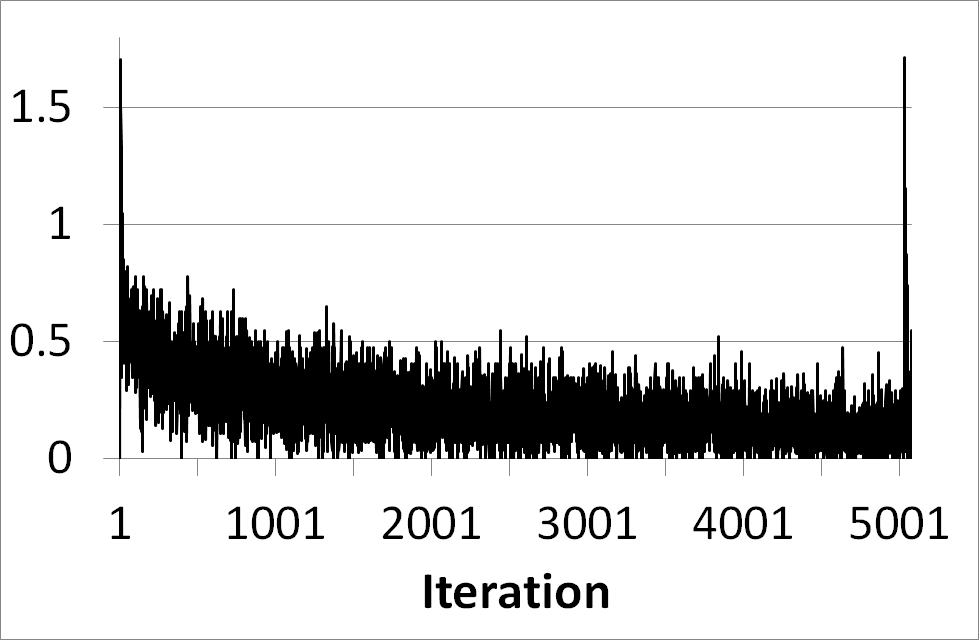
\includegraphics[width=0.95\linewidth]{01b_p3_succ}}
	\label{fig:ImmediateStuckDec3_P3_succ}\hfill
	\subfloat[Global optimum not found]{%
		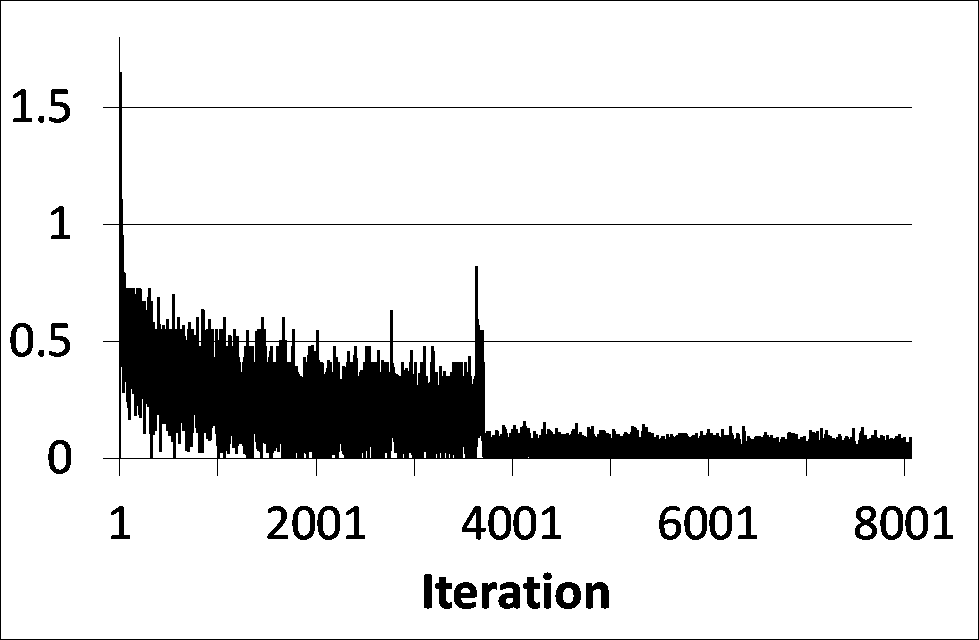
\includegraphics[width=0.95\linewidth]{01_p3_no_succ}}
	\label{fig:ImmediateStuckDec3_P3_fail}\\
	\caption{ The FFE and cache ratio per iteration in exemplary P3 runs (single order-16 standard deceptive function) }
	\label{fig:ImmediateStuckDec3_P3}
\end{figure}

As shown in Fig. \ref{fig:ImmediateStuckDec3_P3}, at the beginning of the run the number of FFE is much higher than the number of successful cache uses. However, the longer the run is, the lower is the FFE cache ratio which means that the number of necessary FFE per iteration drops down. In the successful run (Fig. \ref{fig:ImmediateStuckDec3_P3}a) the ratio significantly rises in the last iteration, because the optimum value was found. On the other hand, in the run in which the optimum was not found, the FFE and cache ratio drops to values that are near to zero. The reason is that at some point the cache becomes large enough to optimize new individuals with FIHC without performing new fitness evaluations, but using cache only.\par


The second considered test case is a single bimodal order-16 deceptive function. Similarly as in the previous case, for such a problem the population of 1000 individuals is usually too small to find the optimal solution (built only from '0's or only from '1's). Therefore, all methods are caught in the local optima containing 8 '0's and 8 '1's. However, since the number of local optima is \begin{math} {8}\choose{8 / 2} \end{math}, the population is not homogeneous as in the previous case. Similarly, DSMGA-II, DSMGA-IIe, and LTGA were usually unable to find the global optimum. The runs in which they succeeded were ignored because they were not interesting (if a global optimum was found it was usually done in the first iteration). The general results for this test case are presented in Table \ref{tab:ImmediateStuckBimod16}.


\begin{table}[]
	\centering
	\caption{FFE and cache - the results for a single order-16 bimodal deceptive function}
	\label{tab:ImmediateStuckBimod16}
	\begin{tabular}{lllll}
		\toprule
		\textbf{Method} & \pbox{20cm}{\textbf{Total FFE}\\\textbf{if no cache}} & \pbox{20cm}{\textbf{Cached}\\\textbf{FFE}} & \pbox{20cm}{\textbf{Population}\\\textbf{cache}} & \pbox{20cm}{\textbf{Iteration}\\\textbf{without}\\\textbf{FFE}}  \\ 
		
		\midrule
		\textbf{DSMGA-II} & & & & \\
		\textbf{mean}                  & 1.02E+07      & 99.83\%             & 47.85\%                         & 99.97\% \\
		\textbf{avg}                   & 1.03E+07      & 99.82\%             & 47.40\%                         & 99.98\% \\
		\textbf{st dev.}               & 2.35E+06      & 0.05\%              & 4.25\%                          & 0.00\%  \\
		\textbf{min}                   & 4.36E+06      & 99.58\%             & 24.48\%                         & 99.97\% \\
		\textbf{max}                   & 1.67E+07      & 99.89\%             & 65.58\%                         & 99.98\% \\
		\midrule
		\textbf{DSMGA-IIe} & & & & \\
		\textbf{mean}                  & 5.95E+06      & 99.70\%             & 48.65\%                         & 99.98\% \\
		\textbf{avg}                   & 6.18E+06      & 99.68\%             & 46.51\%                         & 99.98\% \\
		\textbf{st dev.}               & 1.35E+06      & 0.07\%              & 4.55\%                          & 0.01\%  \\
		\textbf{min}                   & 3.93E+06      & 99.52\%             & 33.15\%                         & 99.96\% \\
		\textbf{max}                   & 9.41E+06      & 99.80\%             & 54.63\%                         & 99.99\% \\
		\midrule
		\textbf{LTGA} & & & & \\
		\textbf{mean}                  & 4.67E+08      & 99.99\%             & 39.22\%                         & 87.02\% \\
		\textbf{avg}                   & 4.68E+08      & 99.99\%             & 39.15\%                         & 86.72\% \\
		\textbf{st dev.}               & 2.09E+07      & 0.00\%              & 0.25\%                          & 2.73\%  \\
		\textbf{min}                   & 4.10E+08      & 99.98\%             & 37.86\%                         & 80.03\% \\
		\textbf{max}                   & 5.12E+08      & 99.99\%             & 39.56\%                         & 92.65\% \\
		\midrule
		\textbf{P3} & & & & \\
		\textbf{mean}                  & 1.29E+05      & 74.08\%             & 38.56\%                         & 0.00\%  \\
		\textbf{avg}                   & 4.43E+05      & 78.73\%             & 37.62\%                         & 8.57\%  \\
		\textbf{st dev.}               & 6.15E+05      & 11.67\%             & 6.39\%                          & 16.33\% \\
		\textbf{min}                   & 7.99E+02      & 61.08\%             & 28.53\%                         & 0.00\%  \\
		\textbf{max}                   & 3.16E+06      & 97.93\%             & 57.17\%                         & 74.05\% \\
		\bottomrule
	\end{tabular}
\end{table}

As presented in Table \ref{tab:ImmediateStuckBimod16}, the percentage of iterations for which no fitness evaluation is done remains significantly high for DSMGA-II and DSMGA-IIe. It shows that for the considered test cases if any of these two methods is stuck then it is hardly capable of searching for new solutions. The similar observation applies to LTGA. For P3 the above observation is not true. Since P3 dynamically adds new individuals during the method run, it is more likely to jump out from the local optimum. Nevertheless, the percentage of cached FFE is very high for all considered methods - close to 100\% for DSMGA-II, DSMGA-IIe, LTGA, and no less than 61\% for P3 in all runs.\par

The percentage of population cache use was similar for all of the considered methods. Usually, it was about 40\% (LTGA and P3) or 50\% (DSMGA-II and DSMGA-IIe) of all successful cache usages. It is an important observation since population cache is easier to use and requires significantly less memory.\par

In this subsection, we have considered two test cases for which considered methods are almost immediately stuck. The first one shows that it is possible, that from some moment method does not generate any fitness computation requests at all. The reason in the case of DSMGA-II and DSMGA-IIe is that no linkage is generated, while in LTGA case the crossed individuals are identical and do not generate any new genotype. For the second test case all methods are stuck and, except P3, are unable to generate any new genotypes. In such situation, the use of fitness caching significantly reduces the necessary FFE. For DSMGA-II and DSMGA-IIe the percentage of method iterations without any new fitness computation is almost 100\%, for LTGA it is over 80\%. Thus, it is allowed to state that fitness caching significantly optimizes the FFE used by these three methods. However, for both of the considered test cases, after the first few iterations DSMGA-II, DSMGA-IIe, and LTGA are stuck and do not require any FFE. Thus, FFE is not a reliable stop condition in these cases.

\subsection{Main Results}
\label{sec:MainResults}

In the previous subsection, we have used two simple test cases to show what may happen when the method is stuck. In this subsection, we will consider regular test problems for evolutionary methods. The experiments are divided into two groups. In the first one, both fitness caching techniques are used. In the second group, only population fitness caching is used.

\subsubsection{Experiments with brutal and population caching}

In this subsection, we present the analysis of experiments designed to check how fitness caching influences the methods applied to solve problems built from deceptive functions concatenations. In Table \ref{tab:cachingInRegularDecBMConcatenations} we show the results for 1200-bit concatenation of order-4 bimodal deceptive functions and the 2400-bit concatenation of order-3 standard deceptive function. The computation time was two hours; each experiment was repeated 10 times. The population size all methods except P3 was 1000.

\begin{table}[]
	\centering
	\caption{Fitness caching statistics for standard and bimodal deceptive functions concatenations}
	\label{tab:cachingInRegularDecBMConcatenations}
	\begin{tabular}{lllll}
				\toprule
		&     \multicolumn{2}{c}{\pbox{20cm}{\textbf{1200-bit order-4}\\\textbf{bimodal deceptive} }}  &      \multicolumn{2}{c}{\pbox{20cm}{\textbf{2400-bit order-3}\\\textbf{standard deceptive} }}        \\
		& & & & \\
		& \pbox{20cm}{\textbf{Cached}\\\textbf{FFE}} & \pbox{20cm}{\textbf{Population}\\\textbf{cache}} &
		\pbox{20cm}{\textbf{Cached}\\\textbf{FFE}} & \pbox{20cm}{\textbf{Population}\\\textbf{cache}} \\
				\midrule
		\textbf{DSMGA-II}	&               &              &               &              \\
		\textbf{mean}    & 31.73\%       & 0.48\%       & 27.09\%       & 3.90\%       \\
		\textbf{avg}     & 31.48\%       & 0.45\%       & 27.49\%       & 4.11\%       \\
		\textbf{st dev.} & 1.76\%        & 0.11\%       & 2.24\%        & 0.82\%       \\
		\textbf{min}     & 29.25\%       & 0.24\%       & 24.33\%       & 2.61\%       \\
		\textbf{max}     & 34.86\%       & 0.58\%       & 30.57\%       & 5.55\%       \\
						\midrule
		\textbf{DSMGA-IIe} &               &              &               &              \\

		\textbf{mean}    & 39.78\%       & 0.15\%       & 28.89\%       & 1.48\%       \\
		\textbf{avg}     & 39.31\%       & 0.16\%       & 28.55\%       & 1.48\%       \\
		\textbf{st dev.} & 3.19\%        & 0.02\%       & 1.27\%        & 0.07\%       \\
		\textbf{min}     & 32.58\%       & 0.14\%       & 26.75\%       & 1.40\%       \\
		\textbf{max}     & 43.87\%       & 0.20\%       & 30.43\%       & 1.60\%       \\
						\midrule
		\textbf{LTGA} &               &              &               &              \\

		\textbf{mean}    & 52.54\%       & 73.18\%      & 39.88\%       & 98.74\%      \\
		\textbf{avg}     & 54.61\%       & 71.84\%      & 46.05\%       & 88.06\%      \\
		\textbf{st dev.} & 18.31\%       & 28.84\%      & 13.04\%       & 22.58\%      \\
		\textbf{min}     & 37.29\%       & 43.74\%      & 39.71\%       & 44.90\%      \\
		\textbf{max}     & 73.13\%       & 99.21\%      & 71.27\%       & 98.84\%      \\
						\midrule
		\textbf{P3} &               &              &               &              \\
		\textbf{mean}    & 63.09\%       & 82.15\%      & 17.08\%       & 95.44\%      \\
		\textbf{avg}     & 62.99\%       & 79.14\%      & 29.50\%       & 84.15\%      \\
		\textbf{st dev.} & 11.05\%       & 10.98\%      & 20.25\%       & 20.55\%      \\
		\textbf{min}     & 48.99\%       & 58.85\%      & 11.87\%       & 46.44\%      \\
		\textbf{max}     & 78.37\%       & 92.73\%      & 60.92\%       & 98.17\%  \\
			\bottomrule
	\end{tabular}
\end{table}

As presented Table \ref{tab:cachingInRegularDecBMConcatenations} usually the percentage of cached fitness evaluations is in the range from 25\% up to 40\% for DSMGA-II and DSMGA-IIe. It is significant that for both of these methods the successful use of population cache was low. It is likely that the population size was too small which has caused the method to stuck and low percentage of successful population fitness caching rate.\par

The experiments for LTGA reported the percentage of successful fitness cache uses in the range from 40\% up to 50\%. Most of these successful uses were obtained with the use of population fitness cache (even up to 98\% in the case 2400-bit order-3 deceptive functions concatenation). High successful fitness caching rate was also obtained for P3 applied to 1200-bit bimodal deceptive functions concatenation. The population caching rate was high as well. Significantly different results were obtained only for P3 applied to solve the problem built from standard deceptive functions. The reason for this fact is simple - P3 was the only method that has solved this problem quickly in all runs. Therefore, fitness caching was barely used in these experiments.\par




\begin{figure}[h]
	\centering
	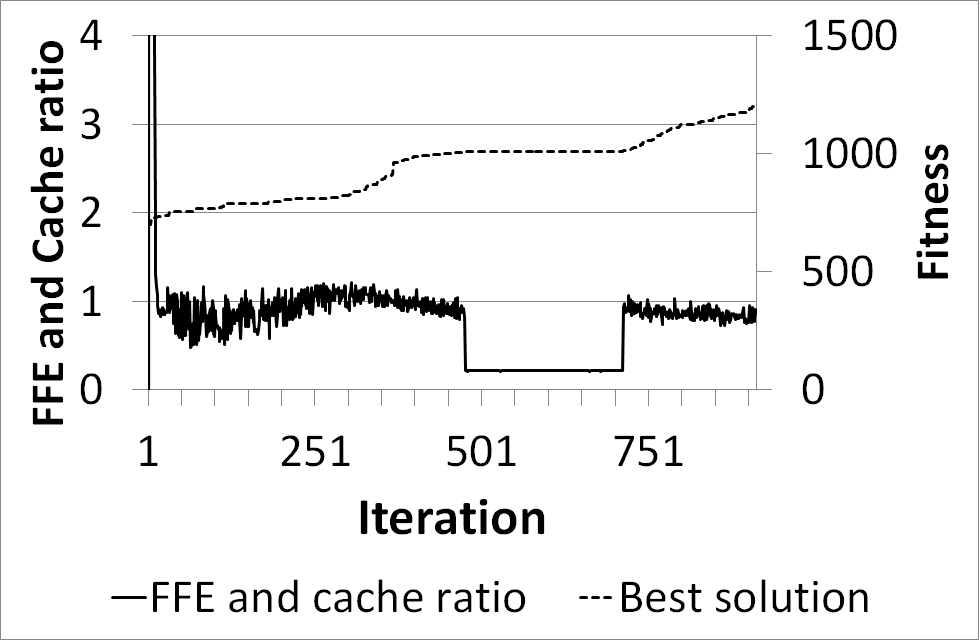
\includegraphics[width=0.98\linewidth]{P3_hole_run}
	\caption{Exemplary P3 run for 1600-bit order-4 bimodal deceptive function concatenation}
	\label{fig:p3_hole_run}
\end{figure}

Fig.\ref{fig:p3_hole_run} presents an exemplary P3 run. The FFE and cache ratio is very high in the first method iterations. It drops down to relatively low values (about 1 - which means that about half of fitness computation requests is computed, the value of other half is returned by successful cache use). Slightly before iteration number 500, the method gets stuck for about 250 iterations - the FFE and cache ratio drops down to values very close to zero (about 0.2), the best found individual value does not improve during this time. Then, the FFE and cache ratio gets back to its previous value, and the fitness of the best-found individual rises quickly. P3 is a method that dynamically manages the population size. However, it is interesting if the monitoring of FFE and cache ratio may be a base for dynamic population size setting in other evolutionary methods.\par

The research direction suggested above may potentially lead to the improvement of DSMGA-II. In Fig. \ref{fig:dsmga2_run} we present an exemplary run of DSMGA-II in which the optimal solution was not found. At first, the FFE and cache ratio is high, then it drops down, but rises again with the rise of the best-found individual value. However, since the $50^{th}$ iteration the ratio value slowly drops down, while the best-found individual fitness value remains the same. It is clear that the method was stuck. If DSMGA-II was monitoring the FFE and cache ratio, it could dynamically increase the population size, jump out from the local optima, and start to investigate new solution space regions.


\begin{figure}[h]
	\centering
	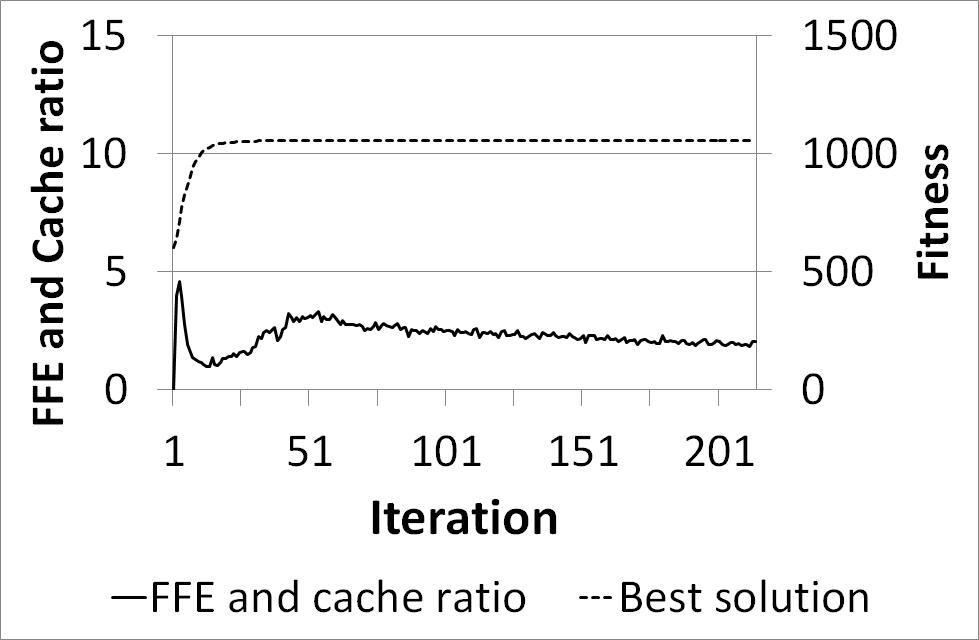
\includegraphics[width=0.98\linewidth]{dsmga2_bm4_1200}
	\caption{Exemplary DSMGA-II run for 1200-bit order-4 bimodal deceptive function concatenation}
	\label{fig:dsmga2_run}
\end{figure}




\subsubsection{Experiments without brutal fitness caching}


\begin{table*}[h]
	\centering
	\caption{FFE and computation time ratio dropdown after method stuck}
	\label{tab:FFE_ratio_dropdown}
	\begin{tabular}{lllrrrrrr}
		\toprule
		&                                 &      & \multicolumn{2}{c}{\pbox{20cm}{\textbf{Until finding}\\\textbf{the best solution}} }     & \multicolumn{4}{c}{\pbox{20cm}{\textbf{After finding the best solution}} }       \\
		\textbf{Method}    & \textbf{Problem}               & \textit{\textbf{n}}    &  \pbox{20cm}{\textbf{ }\\\textbf{FFE/Time}\\\textbf{max [FFE/s]}}    & \pbox{20cm}{\textbf{ }\\\textbf{FFE/Time}\\\textbf{min [FFE/s]}} & \pbox{20cm}{\textbf{ }\\\textbf{FFE/Time}\\\textbf{max [FFE/s]}}    & \pbox{20cm}{\textbf{ }\\\textbf{FFE/Time}\\\textbf{min [FFE/s]}}  & \pbox{20cm}{\textbf{ }\\\textbf{Time}\\\textbf{max [s]}} & \pbox{20cm}{\textbf{ }\\\textbf{Time}\\\textbf{min [s]}} \\ 
		\midrule
		\textbf{DSMGA-II}  & \pbox{20cm}{\textbf{Dec.Conc. Bimodal 10}} & 2000 & 37916.87                              & 17764.84     & 6.42                                  & 17.07        & 42711    & 42446    \\
		\textbf{DSMGA-II}  & \pbox{20cm}{\textbf{ }\\\textbf{HIFF Bimodal 10 (level 3)}}     & 2000 & 60412.73                              & 50334.21     & 314.07                                & 1.76         & 42772    & 42702    \\
		\textbf{DSMGA-IIe} & \pbox{20cm}{\textbf{ }\\\textbf{Dec.Conc. Bimodal 4}}                 & 2000 & 548.15                                & 274.24       & 0.42                                  & \textbf{0.00}         & 32205    & 17819    \\
		\textbf{DSMGA-IIe} & \pbox{20cm}{\textbf{ }\\\textbf{HIFF Bimodal 10 (level 3)}}      & 1000 & 8975.99                               & 7464.18      & 75.52                                 & 2.17         & 39405    & 38707    \\
		\textbf{LTGA}      & \pbox{20cm}{\textbf{ }\\\textbf{Dec.Conc. Step Dec.5 (11-bit)}}  & 1596 & 8286.41                               & 7419.00      & 50.03                                 & 50.03        & 27682    & 27682    \\
		\textbf{LTGA}      & \pbox{20cm}{\textbf{ }\\\textbf{HIFF Bimodal 10 (level 3)}}    & 1000 & 24866.23                              & 17718.92     & 3569.60                               & 2415.37      & 42329    & 41471    \\
		\textbf{P3}        & \pbox{20cm}{\textbf{ }\\\textbf{Dec.Conc. Step Dec.3 (7-bit)}} & 1995 & 1311.19                               & 1018.56      & 1055.61                               & 576.70       & 11084    & 1954    \\ 
		\bottomrule
	\end{tabular}
\end{table*}

In Table \ref{tab:FFE_ratio_dropdown} we present the summarized results of experiments performed for the considered methods on the chosen test cases. The results show the drop down of FFE per second after the last improvement of the best-found individual. The stop condition was set on 12 hours, each experiment was repeated 5 times. The runs in which an optimal solution was found did not affect the results showing the statistics after finding the best solution. The FFE per second ratio drops down most significantly for DSMGA-II, DSMGA-IIe, and LTGA. For all of these three methods, the minimum FFE per second ratio before finding the best solution is about 100 up to 50 000 times higher than after finding the best solution. Note, that for all these cases the minimum computation time after finding the best solution was 5 hours. Thus, the above differences are not accidental. The effect described above is the least significant for P3. This observation is consistent with the results presented in Section \ref{sec:ImmediateStuckExamples} since P3 adds new individual in every method iteration. Therefore, shall not be as vulnerable for being stuck in the local optima as other competing methods.\par

The results reported in Table \ref{tab:FFE_ratio_dropdown} show that sometimes if a method is stuck, it may not cause any fitness computation for a very long time even it uses only population caching. It seems interesting to check how often this phenomenon occurs in some method-test case combinations. Table \ref{tab:100RunsForDSMGA2} presents the FFE per second for DSMGA-II using 3000 individuals solving the 1596-bit concatenation of order-6 bimodal deceptive functions. The stop condition was set on 1 hour. The experiment was repeated 100 times. The table shows the FFE per second ratio before and after the best solution was found. The dropdown is significant - the value decreases almost 4000 times. Note, that most of the computation time was performed with very low FFE per second value.\par


\begin{table}[]
	\centering
	\caption{FFE per second for DSMGA-II (3000 individuals) solving 1596-bit concatenation of order-6 bimodal deceptive functions}
	\label{tab:100RunsForDSMGA2}
	\begin{tabular}{lllll}
		\toprule
		&  \multicolumn{2}{c}{\textbf{Until best}} & \multicolumn{2}{c}{\textbf{After best}}              \\
		& \textbf{FFE/s}    & \textbf{Time {[}s{]}} & \textbf{FFE/s} & \textbf{Time {[}s{]}} \\
		\midrule
		\textbf{mean}       & 36666.90 & 230.50       & 8.48  & 3397.00      \\
		\textbf{avg}        & 38080.65 & 244.45       & 9.62  & 3385.40      \\
		\textbf{st dev.}    & 10625.56 & 91.14        & 8.09  & 86.31        \\
		\textbf{min}        & 12299.93 & 143.00       & 0.00  & 3034.00      \\
		\textbf{max}        & 59445.06 & 688.00       & 33.82 & 3489.00     \\
		\bottomrule
	\end{tabular}
\end{table}

Similar results were obtained for DSMGA-IIe (1500 individuals) applied to solve 1998-bit concatenation of order-6 bimodal deceptive functions (Table \ref{tab:100RunsForDSMGA2e}). The computation time was 8 hours, experimented was repeated 100 times. The FFE per second drops down about 600 times. The values are not accidental since the average computation time before finding the best solution is about six hours, while the computation time after it is over two hours.\par


\begin{table}[]
	\centering
	\caption{FFE per second for DSMGA-IIe (1500 individuals) solving 1998-bit concatenation of order-6 bimodal deceptive functions}
	\label{tab:100RunsForDSMGA2e}
	\begin{tabular}{lllll}
		\toprule
		&  \multicolumn{2}{c}{\textbf{Until best}} & \multicolumn{2}{c}{\textbf{After best}}              \\
		& \textbf{FFE/s}    & \textbf{Time {[}s{]}} & \textbf{FFE/s} & \textbf{Time {[}s{]}} \\
		\midrule
		\textbf{mean}       & 343.24 & 22284.00     & 0.43  & 9158.00      \\
		\textbf{avg}        & 354.19 & 22738.23     & 0.60  & 8857.43      \\
		\textbf{st dev.}    & 80.34  & 4736.89      & 0.54  & 3906.05      \\
		\textbf{min}        & 240.43 & 13075.00     & 0.00  & 2928.00      \\
		\textbf{max}        & 589.44 & 31876.00     & 2.74  & 18122.00    \\
		\bottomrule
	\end{tabular}
\end{table}


Table \ref{tab:TimeAfterTotalStuck} presents the statistics for the runs in which after finding the best solution no fitness was computed until the end of the run. Although the percentage of such runs is low, these results are not accidental - the computation time without any fitness value computation was close to one hour in the case DSMGA-II applied to solve 1596-bit order-6 bimodal deceptive function concatenation, and over two hours in the case of DSMGA-IIe solving 1998-bit concatenation. Note, that it is possible that if the FFE was used as a stop condition, the experiments referred in Table \ref{tab:TimeAfterTotalStuck} would never finish.



\begin{table}[]
	\centering
	\caption{Computation time in runs without any FFE after finding last best individual}
	\label{tab:TimeAfterTotalStuck}
	\begin{tabular}{lllllll}
		\toprule
		&  &          \multicolumn{5}{c}{\textbf{Time {[}s{]}}} \\
		& \pbox{20cm}{\textbf{No}\\\textbf{of}\\\textbf{runs}} & \textbf{mean}    & \textbf{avg}     & \textbf{st dev.} & \textbf{min}     & \textbf{max}     \\
		\midrule
		\pbox{20cm}{\textbf{DSMGA-II}\\\textbf{3000 ind}\\\textbf{1596 bits}}     & 3              & 3458 & 3437 & 42      & 3389 & 3465 \\
		 &                &         &         &         &         &         \\
		\pbox{20cm}{\textbf{DSMGA-IIe}\\\textbf{1500 ind}\\\textbf{1998 bits}}    & 1              & 9371 & 9371 & N/A     & 9371 & 9371 \\
		\bottomrule
	\end{tabular}
\end{table}


\subsection{Results Discussion}

In the results presented in this paper, we show the drop down of the FFE per second ratio caused by fitness caching. We show that for the considered test case-method combinations the change is significantly high. The situation in which a method does not require even a single fitness computation during hours of work leaves no doubt that FFE is not an appropriate computation load measure in this case. Note, that the computation load necessary to compute a single fitness value, does not have to be always enormously large. For instance, for a hard computational problem from the field of computer networks, the average number of FFE per second is in the range from about 40 up to over 400 times ~\cite{MuPPetSeon}. Thus, the FFE-based stop condition may be unfair because the cost of method activities other than fitness computation also significantly affects the overall computation load. This shows that the stop-condition of any research in the field of evolutionary computation shall be always discussed and justified. Using any stop condition type (no matter FFE-, time-based or other), without proper justification may lead to low results reliability.\par

The detailed analysis of some exemplary runs leads to the conclusion that an interesting research direction may be the dynamic population size management on the base of FFE and cache ratio. In the performed experiments, the FFE and cache ration decreases when the method is stuck. Such observation is an expected one - when an evolutionary method is stuck, it tends to check the solutions from already known solution space regions. Thus, the number of successful fitness cache uses shall increase. It is soon to state if the proposed idea will increase the effectiveness of DSMGA-II or LTGA. Nevertheless, it remains promising.\par


time and FFE


\section{Conclusions}

In this paper, we present that a small technical issue, namely the fitness caching, may significantly affect the behavior of evolutionary methods. The main conclusions and future research directions are given below.

\begin{itemize}
	\item The source code quality may significantly affect the number of FFE used by a method - if the method uses fitness caching then, the FFE may be significantly lower than without it.
	\item Population fitness caching always seems to be a reasonable choice. It does not have high computation load requirements and is simple to program. Moreover, some of the results presented in this paper show that population fitness caching may significantly decrease FFE (e.g., in experiments with LTGA solving the 1200-bit order-4 bimodal deceptive functions concatenation and 2400-bit standard deceptive functions concatenation, population fitness caching has decreased the FFE by about 40\%).
	\item In general, FFE shall not be used as a stop condition without justification. For instance, FFE may be unfair if fitness caching is used.
	\item When FFE is used as a computation load measure, and fitness caching is used, then it seems reasonable to use time as an additional stop condition, to assure that the method at least will stop after being stuck.
	\item The monitoring of FFE and fitness cache ration seems to be a promising research direction for dynamic population size management for methods like DSMGA-II and LTGA.
\end{itemize}

The analysis proposed in this paper is a research starting point rather than the complete addressing of issues brought by the fitness caching. Thus, further fitness caching investigation, including test cases based on practical problems instances shall be the main objectives of the future research.


\begin{acks}
	Acks
\end{acks}